\section{PSyclone optimisation for annexed dofs}

The parallel code generated by the PSyclone tool can be modified by
PSyclone configuration options and by bespoke transformation scripts
that can apply to parts of the code or the whole code. This section
describes a change to the code generated by PSyclone and the benefits
it delivered.

The LFRic data model has a concept of ``annexed dofs''. Annexed dofs
relate to data points that are shared between cells owned by two or
more different distributed memory partitions. This is illustrated in
Figure~\ref{fig:dofownership} which shows four partitions {\tt P0} to
{\tt P3} and in particular the halos and dofs for Partition 1. In this
image, the ``Owned dof'' shared by owned cells 3 and 7 in Partition 1
also exists as a dof in the cells 2 and 6 owned by Partition 0.

When a halo swap is done, the infrastructure needs to have defined
which partition holds the correct value for such shared
dofs. Assignment of ownership of these shared dofs is done as part of
the mesh partitioning algorithm at the start of the run. Where a
partition has shared dofs which it does not own, the dofs are referred
to as annexed dofs

Somewhat arbitrarily, ownership of shared dofs is assign to the
partition with the highest number which leads, in the example figure
to Partition 1 owning the dof that it shares with Partition 0. On the
other hand, the dof marked ``Annexed dof'', which is shared with all
four partitions, is owned by Partition 3 and is therefore an annexed
dof in all other partitions including Partition 1.

\begin{figure}[ht!]
\begin{center}
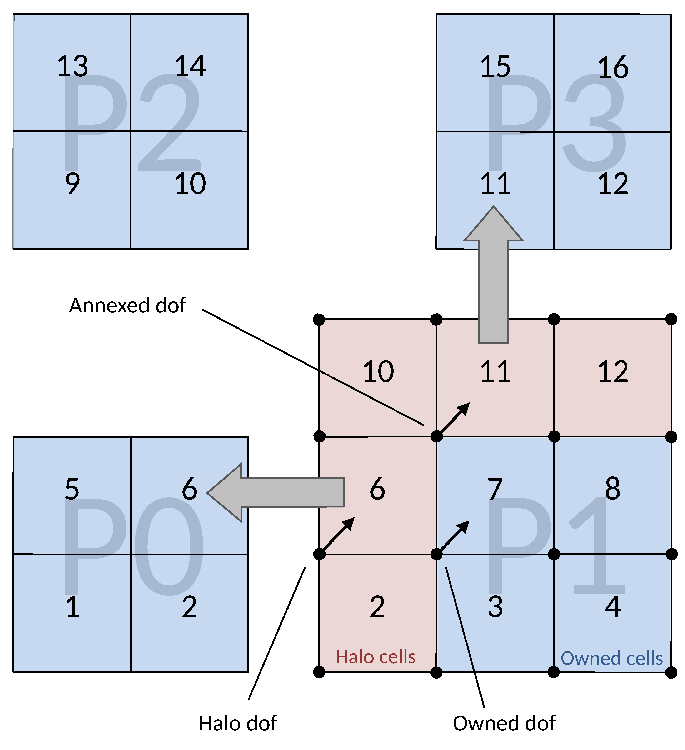
\includegraphics[scale=0.6]{figs/DofOwnership.eps}
\caption{Illustration of owned and annexed dofs. When a halo swap
  occurs Partition 0 will receive the value of the owned dof in
  Partition 1 and the annexed dof in Partition 1 will receive the
  value of the matching dof in Partition 3.}
\label{fig:dofownership}
\end{center}
\end{figure}

While science kernels are computed by looping over cells, PSyclone
supports a number of ``built-in'' operations that are computed by
looping over dofs. Such operations include initialisation of fields
and basic arithmetic operations such as adding fields or multiplying
fields by scalar values. Originally, the strategy applied by PSyclone
was to compute only the owned dofs and not the annexed dofs. The
assumption was that a halo swap would always be needed before a
built-in result would be used, and therefore computing the annexed
dofs was unnecessary.

Later it was recognised that there were operations which would not
require halo values of fields, and therefore the option was made to
compute the annexed dofs and to remove unnecessary calls to halo swap
routines.

The impact of this change was assessed and the description of the
experiment and results follows.

\subsection{Method}

The version of the trunk used in these tests was 17655 but with the same science configuration as
used in~\ref{sec:scale},
%The version of the trunk and GungHo C576 GungHo configuration that was
%assessed in \ref{sec:scale} was used for these tests, 
running on
the Cray XCS using the LFRic environment built for the Intel compiler
version 17.0.0.098. Configurations were run on 24, 54 and 96 nodes
with 6 OpenMP threads per rank. 

The difference between the control and test runs was a PSyclone
configuration setting that, by default, modified the loop limits for
all built-ins to loop either over owned dofs or over annexed dofs.
Additionally, following some initial trials and analysis, the standard
optimisation script within GungHo was modified to override this
default for those built-ins which initialise new fields: {\tt
  setval\_c} and {\tt setval\_x} which respectively initialise a field
to a constant value, and set the value of one field to another. This
additional change prevents uninitialised halo data being accessed when
a newly initialised continuous field is passed into a kernel which
increments its value. The setting will become the default for a future
version of PSyclone.

\subsection{Results and analysis}

The questions to be answered are: what impact does this change have on
the number of halo swaps required and what is the cost in time saved
from reduced halo swaps relative to the increase in time for the extra
calculations.

For an example field in the 96-node job, the number of owned and
annexed dofs was 318,096. The number of annexed dofs varies from
partition to partition, but the maximum number was 7200. This equates
to 2.2 percent additional redundant computation for annexed dof
operations which likely comprise a minority of the total cost of
computation. As the PSyclone-generated loops that implement the
built-in operations are scattered through the PSy layer code it is not
currently possible to add instrumentation to measure their cost.

LFRic infrastructure enables the number of halo swaps to be
counted. For the two scenarios, the number of halo swaps was reduced
by 52\% from 9120 per time-step for the control job to 4360 per
time-step.  Table~\ref{tab:annex} lists the cost of the halo swaps in
each of the tasks recorded by Cray PAT as the cost of the
\verb+xt_exchanger_mix_isend_irecv_s_exchange+. As can be seen, the
savings should comfortably outweigh the cost of the redundant
computation.


\begin{table}[ht!]
\scriptsize
  \begin{center}
    \caption{Percentage cost of halo swap}
    \label{tab:annex}
     \begin{tabular}{|c|c|c|}
      \textbf{Nodes} & \textbf{Original} & \textbf{Annexed dofs} \\
      \hline
      24 & 5.3  & trace  \\ 
      54 & 8.7  & 3.4    \\ 
      96 & 10.7 & 4.8    \\ 
      216 & 12.0 & -    \\ 
      384 & 13.0 & -    \\ 
    \end{tabular}
  \end{center}
\end{table}

Note that the cost of a single halo swap rises with the increase in
node count, and while the annexed dof version was not re-run on larger
node counts, the figures from the control run are listed in the table
to give an idea of the likely benefit. 





